\documentclass[12pt]{report}
\usepackage[T2A]{fontenc} 
%\usepackage[cp1251]{inputenc}
\usepackage[utf8]{inputenc}
\usepackage[russian, english]{babel}
\usepackage{cmap}
\usepackage{xkeyval}
\usepackage[pdftex]{graphicx}
\usepackage{amsmath}
\usepackage{amsfonts}
\usepackage{multirow}
\usepackage{xfrac}
\usepackage[labelformat=empty]{caption}
\usepackage[left=2cm,right=2cm,
     top=2cm,bottom=2cm,bindingoffset=0cm]{geometry}
     %\geometry{margin=1cm}%Just for showing, these are bad margins!
%\usepackage[pdftex]{graphics}
\graphicspath{{images/}}
\frenchspacing

%4 listing 

\usepackage{listings} %% собственно, это и есть пакет listings
\usepackage{color} %% это для отображения цвета в коде
\definecolor{mygreen}{rgb}{0,0.6,0}
\definecolor{mygray}{rgb}{0.5,0.5,0.5}
\definecolor{mymauve}{rgb}{0.58,0,0.82}
\tolerance=1000

\usepackage{caption}
\DeclareCaptionFont{white}{\color{white}} %% это сделает текст заголовка белым
%% код ниже нарисует серую рамочку вокруг заголовка кода.
\DeclareCaptionFormat{listing}{\colorbox{black}{\parbox{\textwidth}{#1#2#3}}}
\captionsetup[lstlisting]{format=listing,labelfont=white,textfont=white}

\usepackage{etoolbox}
\makeatletter
\patchcmd{\chapter}{\if@openright\cleardoublepage\else\clearpage\fi}{}{}{}
\makeatother


\begin{document}

\righthyphenmin=2
\newpage
\hfill \text{Серебро Андрей, студент  43601/2}\\

\section* {Расстояние Канторовича на графе Юнга}
\parindent=1cm
\newenvironment{myindentpar}[1]%
 {\begin{list}{}%
         {\setlength{\leftmargin}{#1}}%
         \item[]%
 }
 {\end{list}}
 
\subsection*{Нумерация двумерных диаграмм}
\hspace{\parindent} Повторены результаты предшественников по части нумерации двумерных диаграмм Юнга. 

Обозначим: 

\begin{itemize}
  \item $\No(\lambda)$  - номер диаграммы $\lambda$
  \item $Cells(\lambda)$  - число клеток в $\lambda$
  \item $h_\lambda(i)$ - высоту столбца с номером $i$ в диаграмме $\lambda$ (высоты считаем положительными целыми числами)
  \item $r_\lambda(i)$ - длину строки с номером $i$ в диаграмме $\lambda$
  \item $Cols(\lambda)$ - число столбцов в диаграмме $\lambda$
  \item $Y_n$ - множество двумерных диаграмм Юнга из $n$ клеток
\end{itemize}
Нумерация удовлетворяет следующим трём правилам:\\
1. Номер диаграммы из одной клетки равен 1;\\
2. Если $Cells(\lambda_1) < Cells(\lambda_2)$, то $\No(\lambda_1) < \No(\lambda_2)$;\\
3. Иначе если $Cells(\lambda_1) = Cells(\lambda_2)$ и $\exists k \ge 1 : \forall i \in \{1..k-1\} h_{\lambda_1}(i) = h_{\lambda_2}(i)$ и $h_{\lambda_1}(k) < h_{\lambda_2}(k)$, то $\No(\lambda_1) < \No(\lambda_2)$

Для того, чтобы найти номер диаграммы по этим правилам, предварительно подсчитывается $P(n, k)$ $\forall n, k \in \mathbb{N} : 0 < n < N, k < n$ - число разбиений числа $n$ на натуральные слагаемые с максимальным слагаемым, не превосходящим $k$. На данный момент число $N = 600$, так как нумерация диаграмм с большим числом клеток не требуется.

\newpage
\subsection*{Подсчёт расстояния Канторовича между диаграммами}

\hspace{\parindent} Основываясь на статье А. М. Вершика, реализован подсчёт расстояний Канторовича между диаграммами в графе Юнга. В качестве центральной меры на пространстве путей взята мера Планшереля. Проведены эксперименты (в том числе, я выяснил, что за разумное время - около получаса - можно найти расстояние между двумя диаграммами из 50 клеток, при этом пришлось решить 36 695 768 транспортных задач.) Между диаграммами из 40 клеток расстояние ищется за время порядка 30 секунд. Также вычислены все расстояния между диаграммами на 10 этаже графа Юнга, гистограмму расстояний можно увидеть на рис. 3.

\begin{figure}[!ht]
\begin{center}
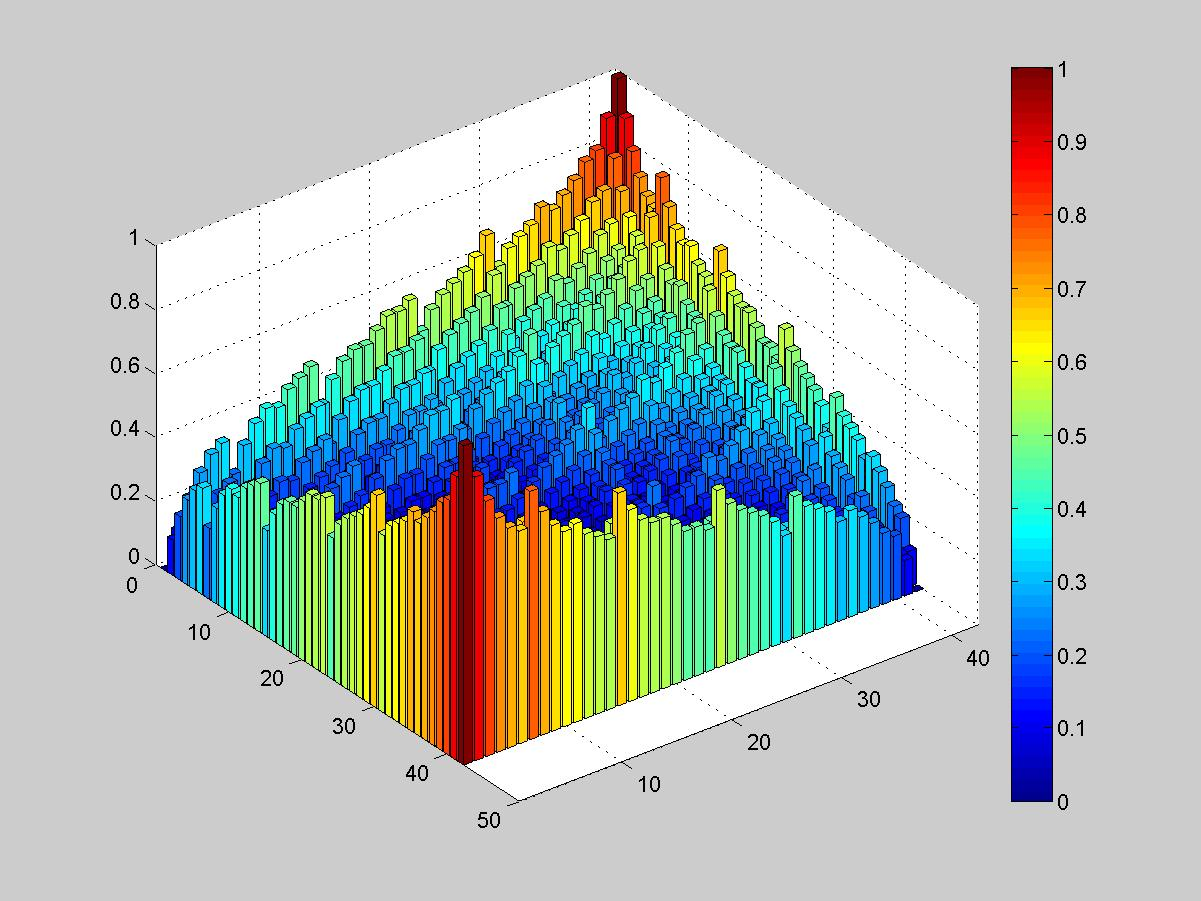
\includegraphics[scale=0.2]{metricHist1}
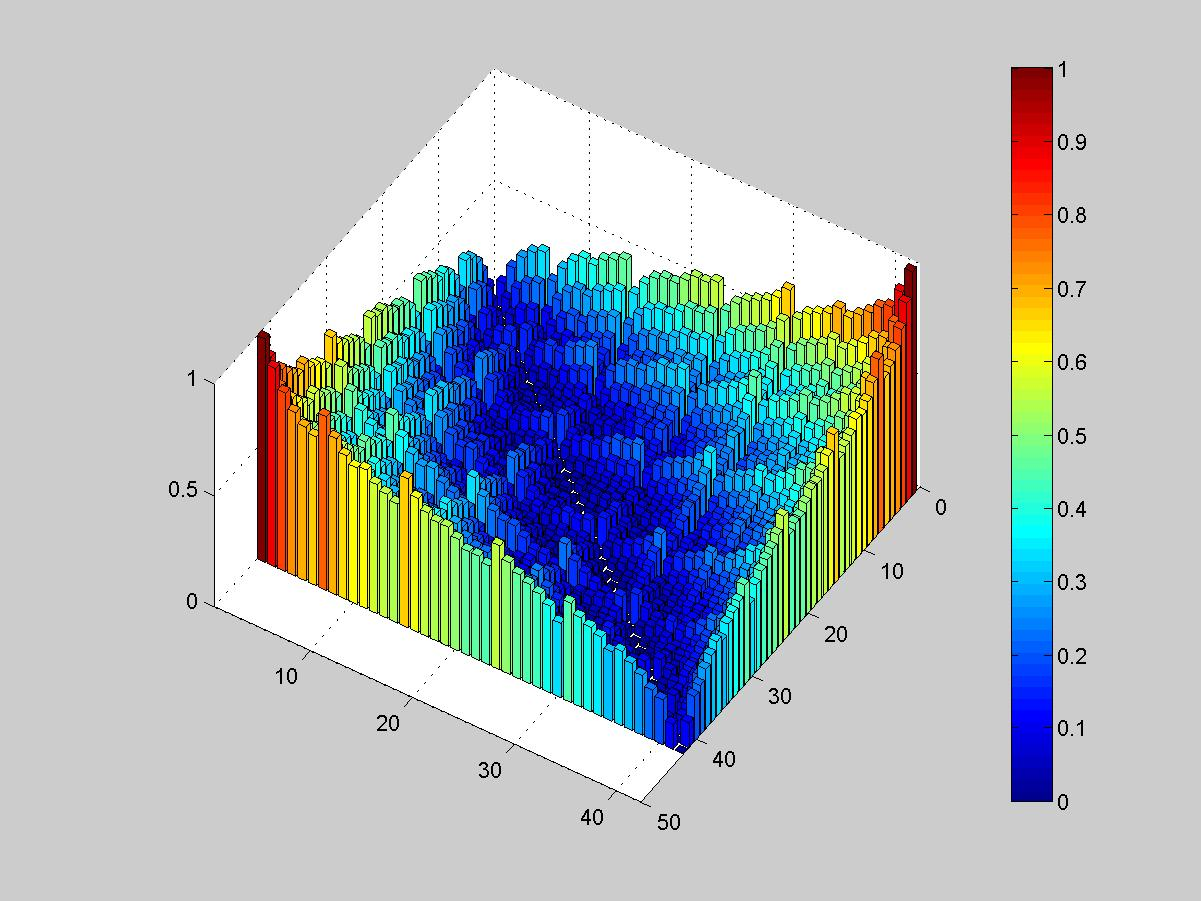
\includegraphics[scale=0.2]{metricHist2}
\\Рис. 3. Гистограмма расстояний Канторовича между диаграммами 10го этажа графа Юнга. 
\end{center}
\end{figure}

Рисунок 4 по сути является сечением описанной выше гистограммы при фиксированном номере одной из диаграмм Юнга, только для случая диаграмм из 20 клеток, а не 10. Графики показывают существенную разницу между граничными диаграммами и случайными диаграммами из 20 клеток: средняя диаграмма, взятая в процессе Планшереля, находится на расстоянии ближе 0.05 от большей части диаграмм. Диаграмма-строка далека от почти всех диаграмм. 

\begin{figure}[!ht]
\begin{center}
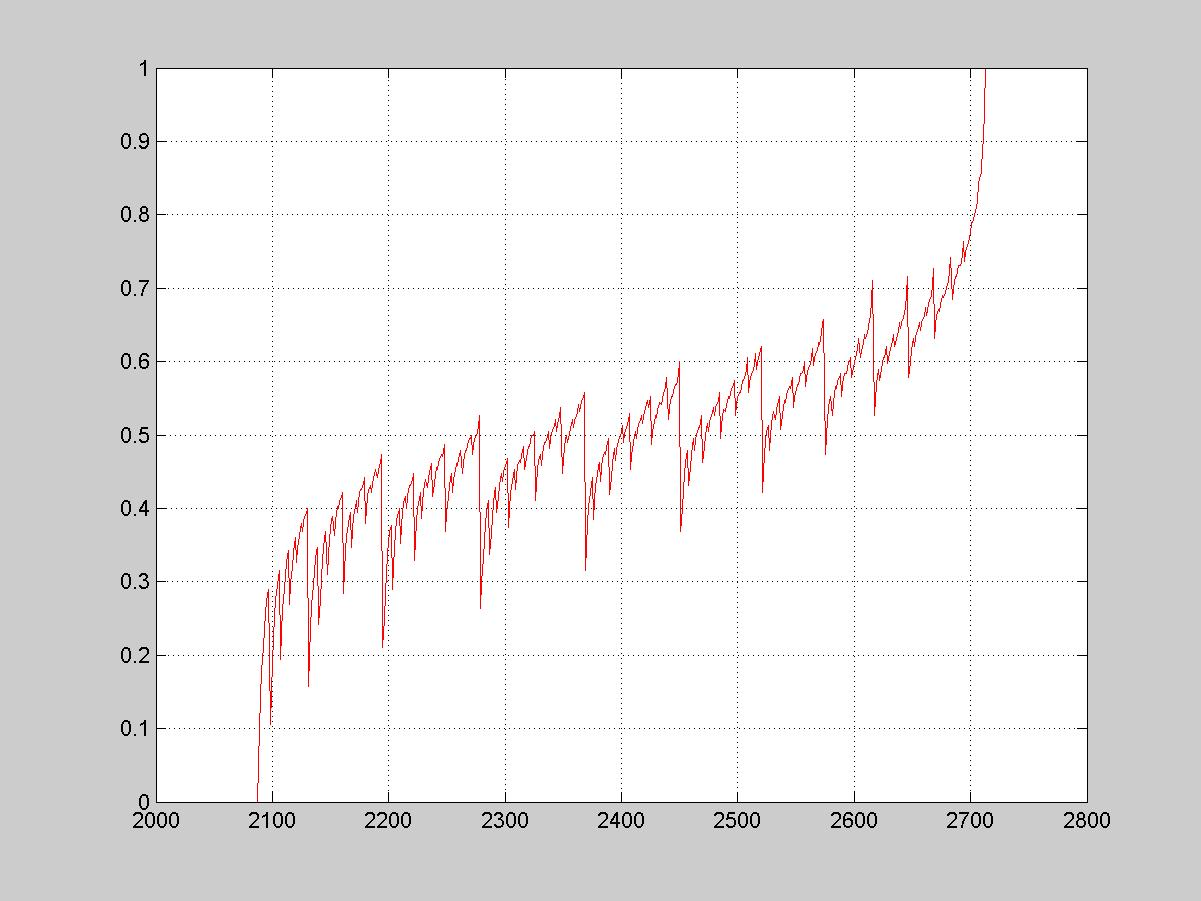
\includegraphics[scale=0.2]{DiagramsDists20FromLine}
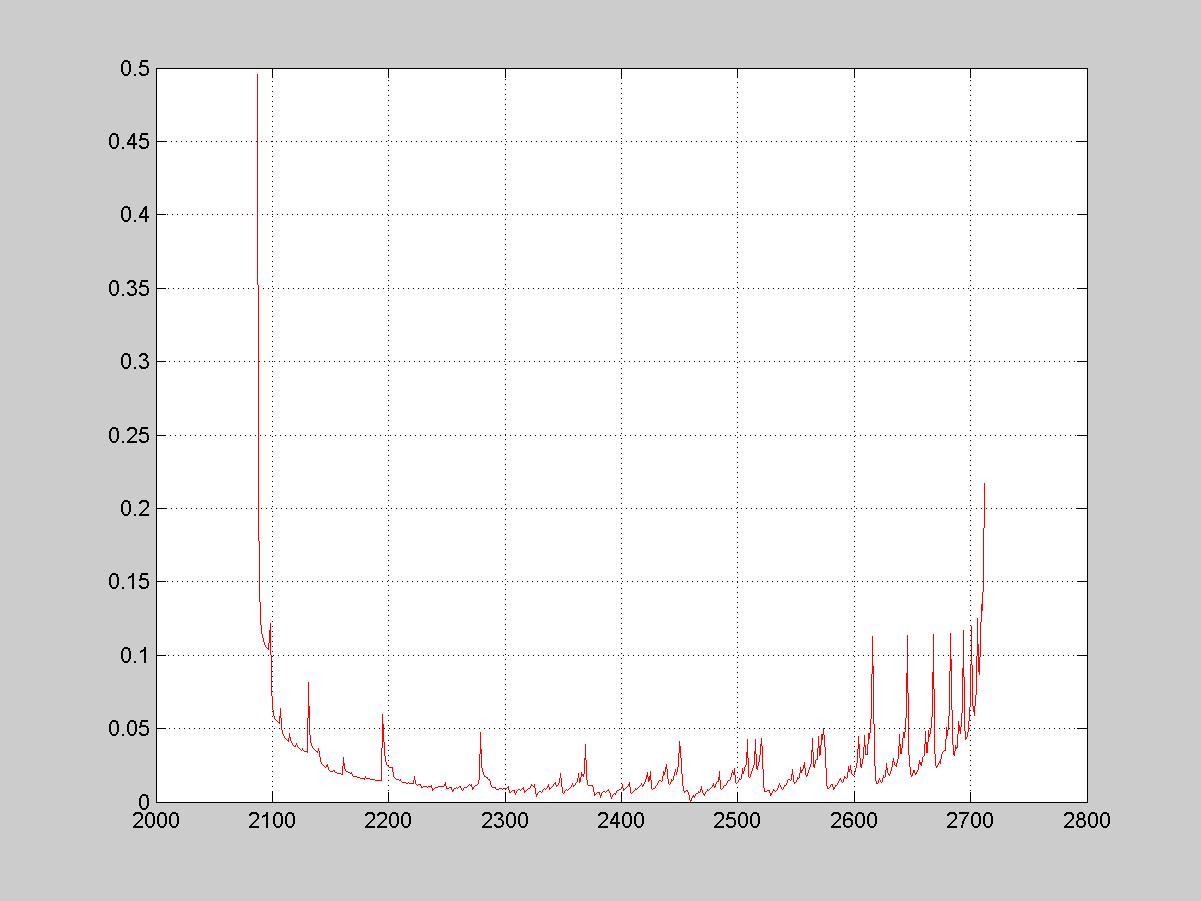
\includegraphics[scale=0.2]{DiagramsDists20}
\\Рис. 4. Расстояния от диаграммы-линии из 20 клеток до всех других диаграмм (слева), и расстояния от случайной диаграммы из 20 клеток до всех остальных (справа)
\end{center}
\end{figure}

\subsection*{Метрика Канторовича на симплексе}

\hspace{\parindent} Для понимания того, как устроена метрика Канторовича, было рассмотрено расширение метрики с вершин симплекса на симплекс. Размерность симплекса выбрана два для наглядности. В результате стало понятно, что в двумерном случае шарами являются шестиугольники. Для этого я выбирал произвольную точку внутри треугольника (например, центр масс) и считал расстояния между ним и узлами сетки, на который предварительно разбил треугольник. Интересен простейший случай, когда треугольник равносторонний, то есть расстояния между всеми вершинами заданы одинаковыми. В этом случае шестиугольники точек, равноудаленных от центра масс треугольника получаются равносторонними со сторонами, параллельными сторонам треугольника (см. рис. 5). Это позволяет также выдвинуть некоторые гипотезы касательно того, как может выглядеть сфера в более высоких размерностях. Немного порисовав, я представил себе, как выглядит шар в трёхмерном случае, когда симплекс - правильный тетраэдр. Это будет четырнадцатигранник, составленный из 8 тетраэдров и 6 четырёхугольных пирамид. Картинку его я смог найти например тут: http://borgece.livejournal.com/1854.html, по запросу четырнадцатигранник. Две нижние картинки показывают метрику на равностороннем треугольнике.
Сейчас хочу попробовать экстраполировать представление шара на произвольную размерность (думаю, будет полезно для понимания структуры  шаров на графе Юнга).

Отталкиваться можно от числа гиперграней шара: число граней в зависимости от размерности выглядит так:

\begin{center}
\begin{tabular}{|c|c|c|c|c|}
\hline
Размерность симплекса & 1 & 2 & 3 & ...\\
\hline
число граней шара & 2 & 6 & 14 & ? \\
\hline
\end{tabular}
\end{center}

Быть может, в пространстве размерности $n$ число граней есть $2 (2^n - 1)$. 

С другой стороны, можно понять и, я полагаю, доказать, что при сечении шара размерности $n$ гиперплоскостями, параллельными сторонам симплекса, будет получаться шар размерности $n - 1$. Когда же сечение дойдёт до границы симплекса, оно даст в пересечении с этой границей просто симплекс размерности $n-1$. Это ещё один способ представить себе шары больших размерностей.
\begin{figure}[!ht]
\begin{center}
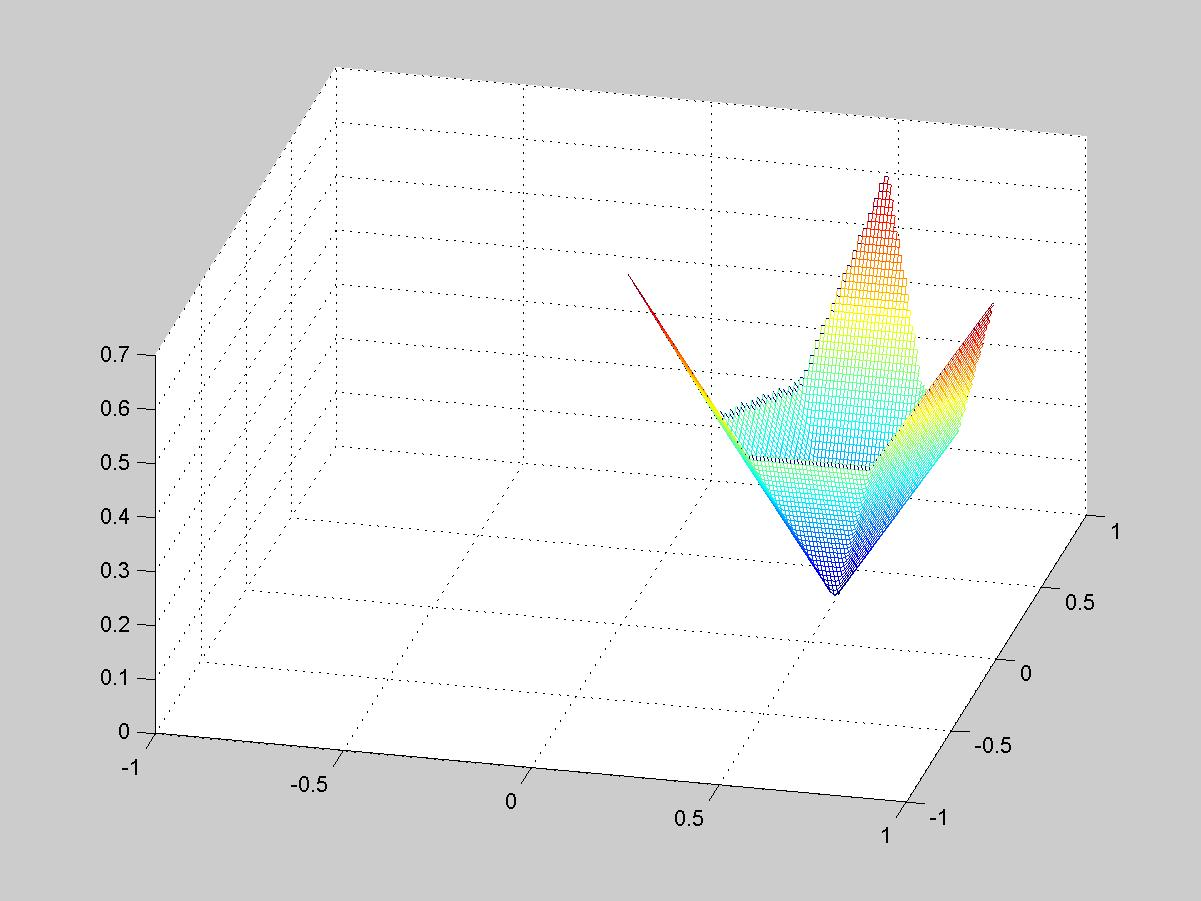
\includegraphics[scale=0.2]{SimplexDists1}
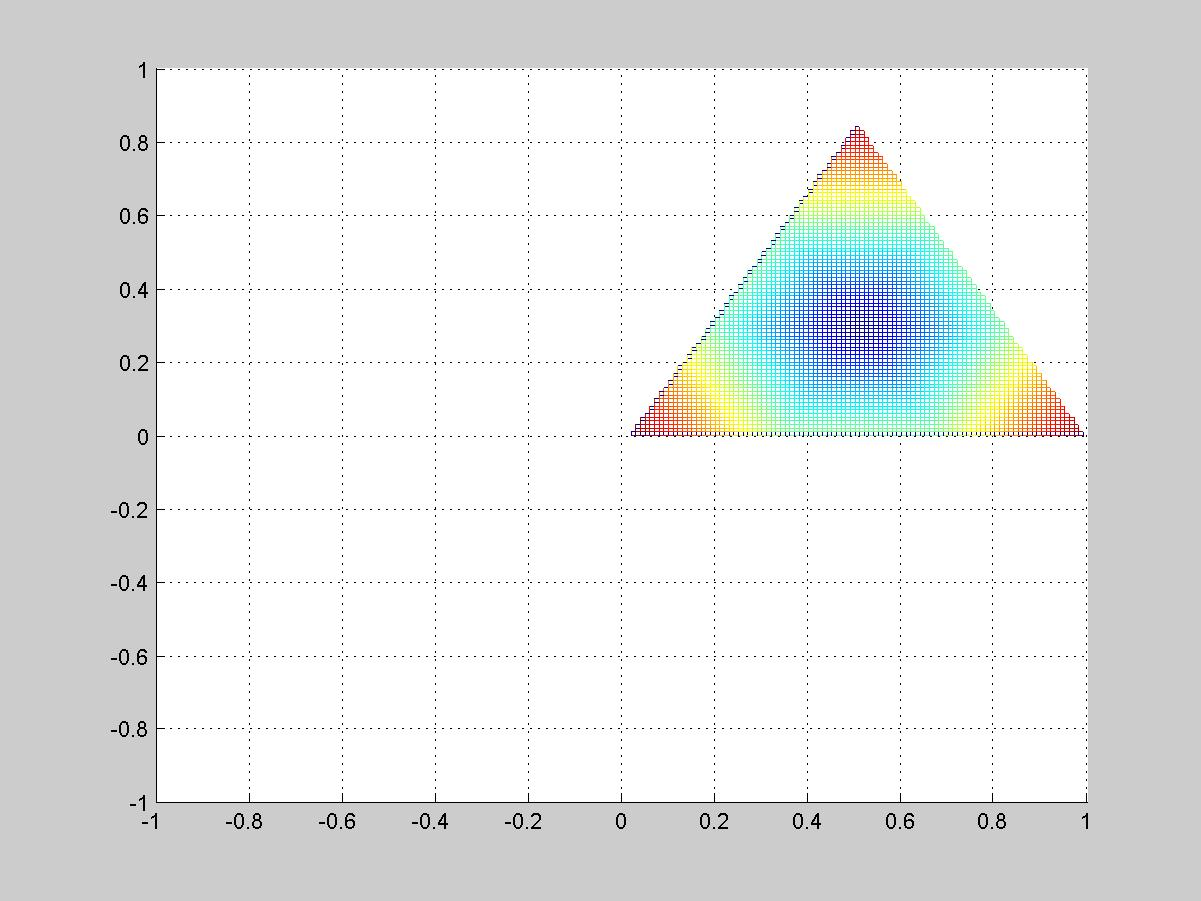
\includegraphics[scale=0.2]{SimplexDists2}
\\Рис. 5. Расстояния между центром масс равностороннего треугольника и точками треугольника. Равноудаленные точки дают одинаковый цвет графика.
\end{center}
\end{figure}


\begin{figure}[!ht]
\begin{center}
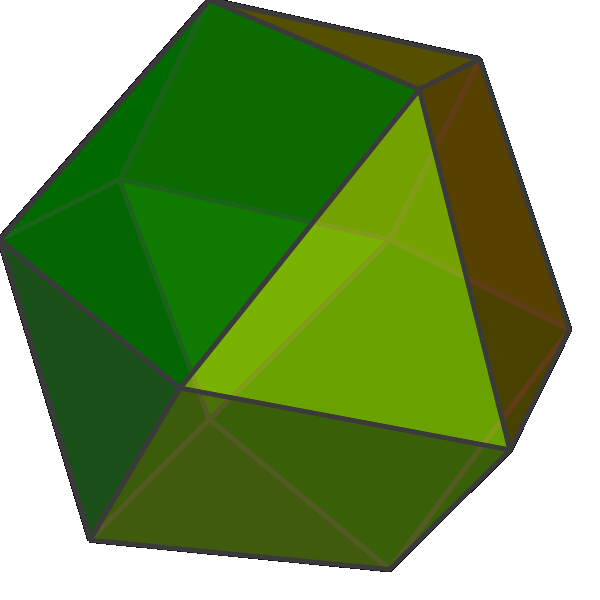
\includegraphics[scale=0.4]{14surf}
\\Рис. 6. Четырнадцатигранник (кубооктаэдр), который является шаром в трёхмерном случае. В случае правильного симплекса все его грани параллельны граням исходного симплекса (тетраэдра).
\end{center}
\end{figure}

\newpage
\subsection*{Приближение метрики Канторовича}
\hspace{\parindent} Рассмотрена гипотеза А. М. Вершика о том, что расстояние Канторовича между диаграммами $dist(\lambda_1, \lambda_2) = \sum\limits_{i = 1}^n c_i\Delta_i$, где $\Delta_i = r_{\lambda_1}(i) - r_{\lambda_2}(i)$, $c_i$ - какие-то коэффициенты, предположительно быстро убывающие с ростом $i$. Предлагается, насколько я понял, попробовать подобрать их, а также убедиться, что коэффициенты действительно быстро убывают:  например, это можно увидеть, рассмотрев расстояние между прямоугольной диаграммой и треугольной, которое видимо будет маленьким, несмотря на их непохожесть, так как первые строки у них будут иметь почти одинаковый размер. 

Сейчас решается несколько более простая задача: оценка расстояния от данной диаграммы до всех других. Приближение ищется методом наименьших квадратов путем минимизации функции невязки. Пусть взята диаграмма $\lambda$, $n = Cells(\lambda)$ и мы хотим оценить расстояние от неё до произвольной диаграммы с её уровня. Для этого решаем задачу: $$c = \arg \min\limits_{c \in \mathbb{R}^n}(\sum\limits_{\lambda_i \in Y_n}(\sum\limits_{j = 1}^n c_j\Delta_{ij} - dist(\lambda, \lambda_i))^2),$$ где $\Delta_{ij} = r_{\lambda}(i) - r_{\lambda_{j}}(i), i = 1..n, j = 1..|Y_n|$.

С результатами можно ознакомиться на рисунке 7 (бралась случайная диаграмма из 20 клеток и считалось расстояние от неё до всех остальных). Видно, что хотя невязка присутствует, имеется явная корреляция между $\Delta_i$ и расстоянием, что позволяет сделать вывод о возможности лучшей оценки с помощью каких-то более сложных функций от $\Delta_i$. Вполне возможно, что для этого достаточно добавить в оценку разницу столбцов, хотя бы ради симметрии. Думаю, это следует попробовать сделать в ближайшее время.

\begin{figure}[!ht]
\begin{center}
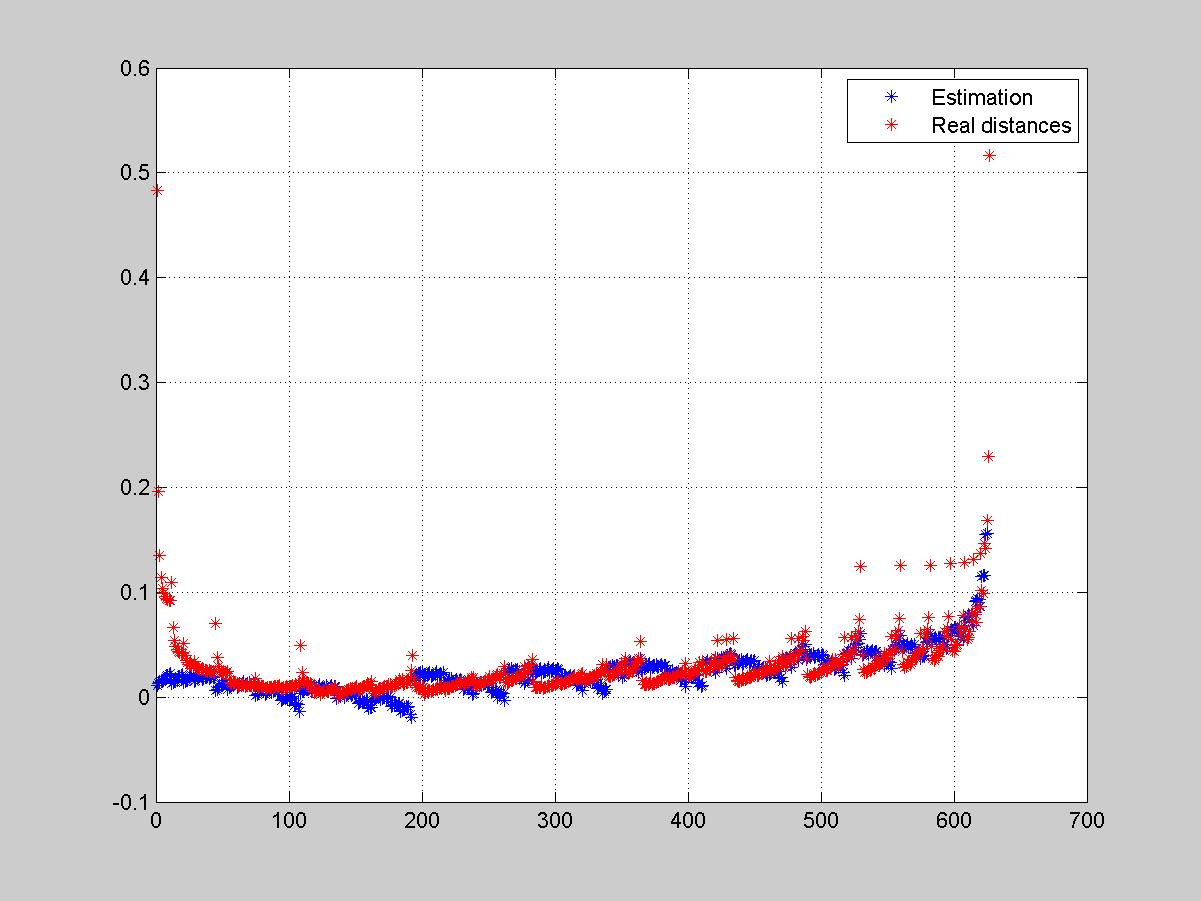
\includegraphics[scale=0.2]{MetricEstimation20}
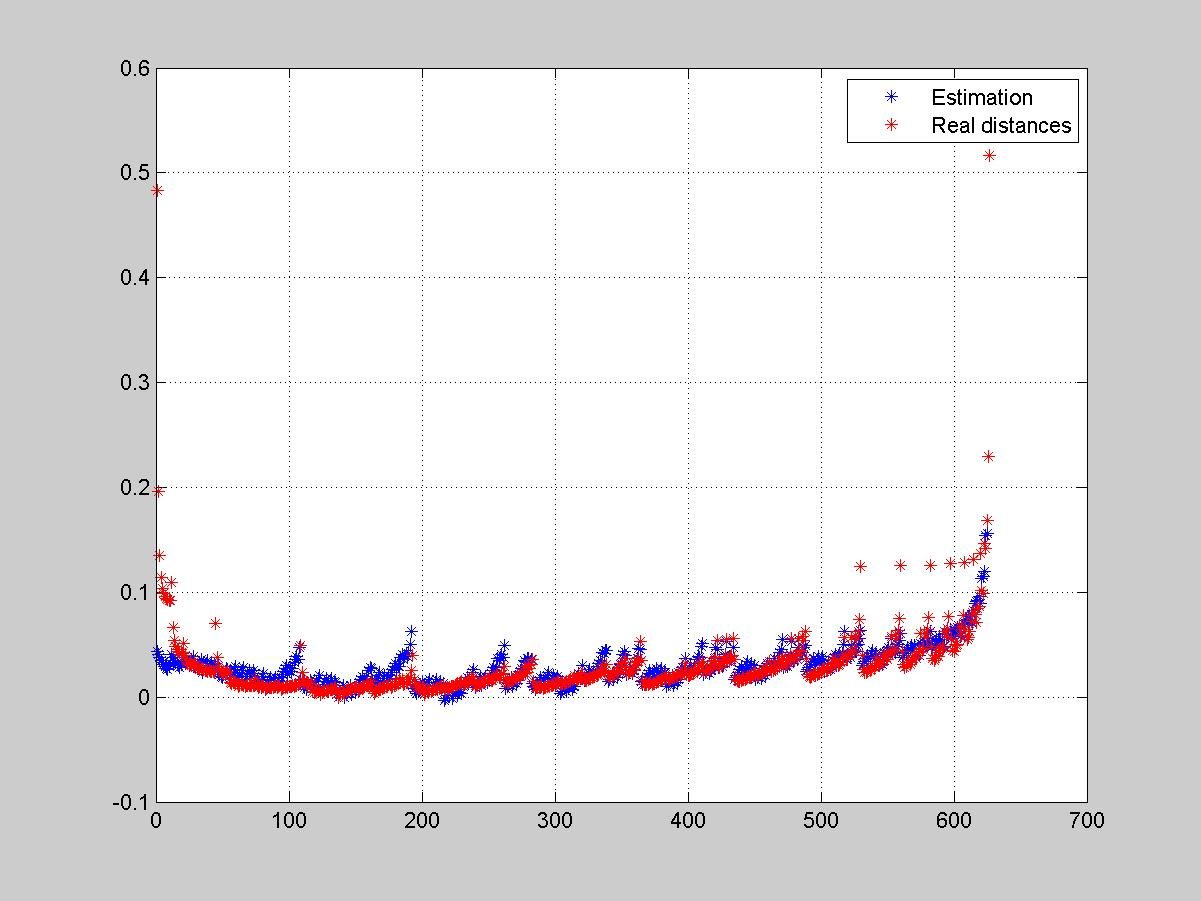
\includegraphics[scale=0.2]{MetricEstimation20Fabs}
\\Рис. 7. Расстояния от некоторой диаграммы до всех других диаграмм и их оценка по МНК. Слева оценка без модуля, справа взята оценка с модулем разниц строк: $dist(\lambda_1, \lambda_2) = \sum\limits_{i = 1}^n |c_i\Delta_i|$
\end{center}
\end{figure}

Посмотрим на вектор коэффициентов для обеих оценок (с модулем и без):
\begin{center}
\begin{tabular}{|c|c|c|c|c|c|c|c|c|c|c|}
\hline
Без модуля &-0.296 & -0.291 & -0.289 &-0.289 &... & -0.308& -0.317& -0.332 &-0.368 &-0.583\\
\hline
C модулем & 0.0193 & -0.0024 & -0.0032& 0.0145&... & 0.0348 & 0.0351& 0.0391& 0.0415& 0.0333   \\
\hline
\end{tabular}
\end{center}

Интересно, что в то время, как первые не меняют знак, вторые его чередуют (в номерах, попавших в многоточие имеется несколько отрицательных коэффициентов). 

На рисунке 8 представлена зависимость коэффициентов $c(i)$ для случая оценки с модулем и без. 
\begin{figure}[!ht]
\begin{center}
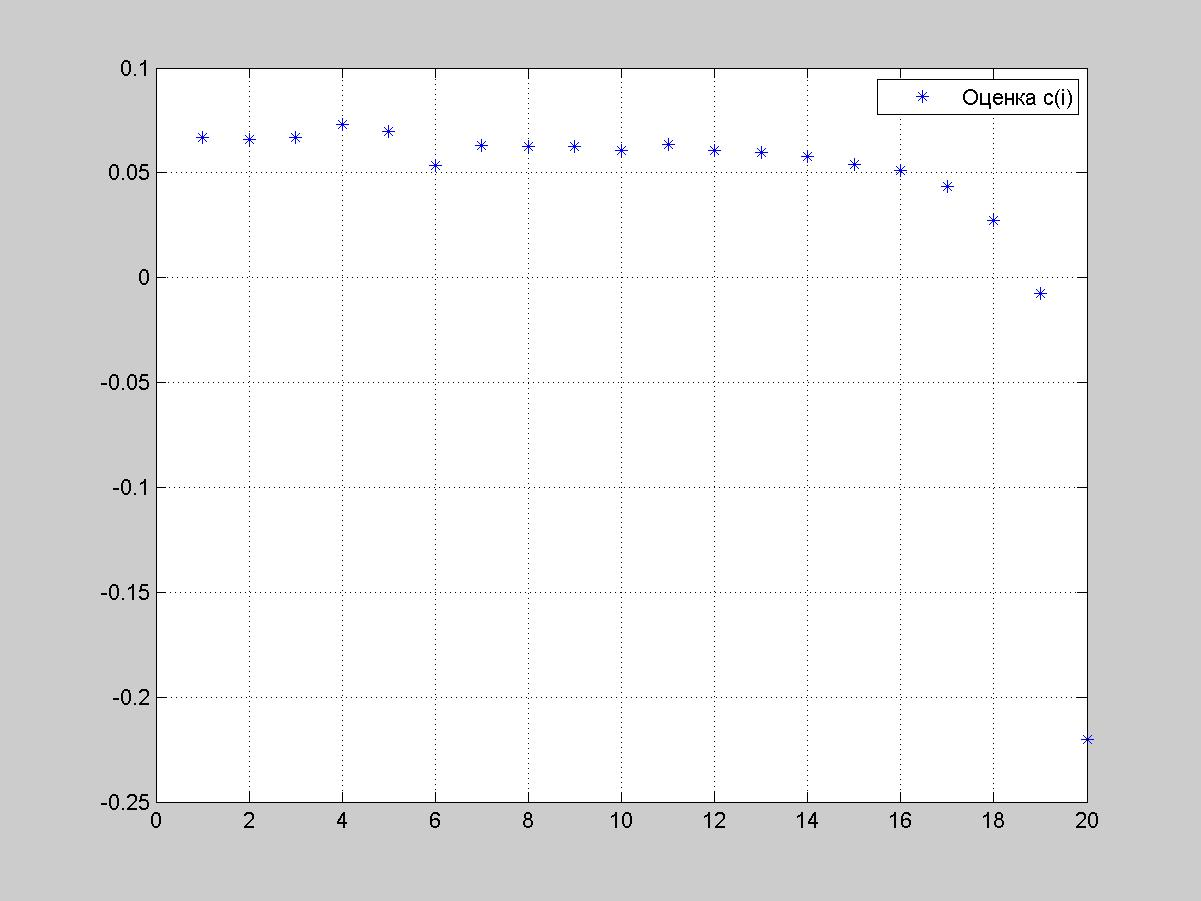
\includegraphics[scale=0.2]{CoefficientsEstimation20}
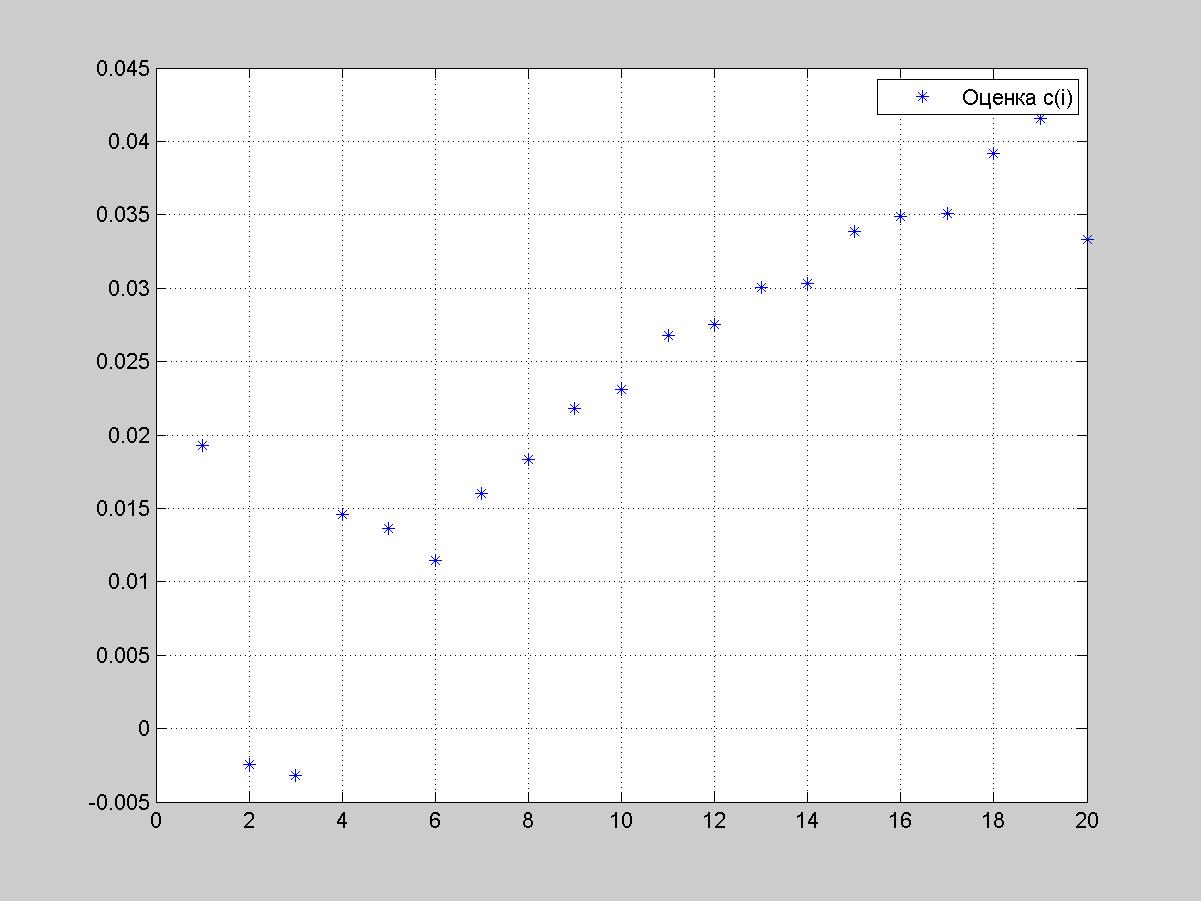
\includegraphics[scale=0.2]{CoefficientsEstimation20Fabs}
\\Рис. 8. Коэффициенты $c(i)$. Слева случай без модуля, справа случай оценки с модулем.
\end{center}
\end{figure}


\end{document}